% This is samplepaper.tex, a sample chapter demonstrating the
% LLNCS macro package for Springer Computer Science proceedings;
% Version 2.20 of 2017/10/04
%
\documentclass[runningheads]{llncs}
%
\usepackage{graphicx}
\usepackage{caption}
\usepackage{subcaption}
% \usepackage{pdfpages}
% Used for displaying a sample figure. If possible, figure files should
% be included in EPS format.
%
% If you use the hyperref package, please uncomment the following line
% to display URLs in blue roman font according to Springer's eBook style:
% \renewcommand\UrlFont{\color{blue}\rmfamily}

% % Dãn dòng 1.5
% \usepackage{setspace}
% \onehalfspacing

% Font tiếng Việt
\usepackage[T5]{fontenc}
\usepackage[utf8]{inputenc}
\DeclareTextSymbolDefault{\DH}{T1}

% Chèn và định dạng mã giả
\usepackage{amsmath}
\usepackage{algorithm}
\usepackage[noend]{algpseudocode}
\makeatletter
\def\BState{\State\hskip-\ALG@thistlm}
\makeatother

% chèn inline code
\usepackage{xparse}
\NewDocumentCommand{\codeword}{v}{%
    \texttt{\textcolor{blue}{#1}}%
}

% equation
\usepackage{breqn}
\usepackage{amsfonts}
\usepackage{bm}

% Bảng biểu
\usepackage{multirow}
\usepackage{float}
\usepackage{makecell}
\usepackage{rotating}
\usepackage{vcell}
\usepackage{array}
\usepackage{diagbox}
\usepackage{booktabs}
\usepackage{colortbl}
\newcolumntype{L}[1]{>{\raggedright\let\newline\\\arraybackslash\hspace{0pt}}m{#1}}
\newcolumntype{C}[1]{>{\centering\let\newline\\\arraybackslash\hspace{0pt}}m{#1}}
\newcolumntype{R}[1]{>{\raggedleft\let\newline\\\arraybackslash\hspace{0pt}}m{#1}}

\begin{document}
%
\title{Meta-learning and Personalization layer \\in Federated learning}
% \title{Meta-learning and Personalization layer \\in Federated learning\thanks{This research is funded by University of Science, VNU-HCM under grant number CNTT 2022 - 09}}
%
% \titlerunning{Abbreviated paper title}
% If the paper title is too long for the running head, you can set
% an abbreviated paper title here
%
\author{Bao-Long Nguyen\inst{1,2}\orcidID{0000-0002-6411-8943} \and
Tat Cuong Cao\inst{1,2}\orcidID{0000-0003-1803-843X} \and Bac Le\inst{1,2}\thanks{Corresponding Author}\orcidID{0000-0002-4306-6945}}
%
\authorrunning{B.L. Nguyen et al.}
% First names are abbreviated in the running head.
% If there are more than two authors, 'et al.' is used.
%
\institute{Faculty of Information Technology, University of Science, Ho Chi Minh City, VietNam \and VietNam National University, Ho Chi Minh City, VietNam}
%
\maketitle              % typeset the header of the contribution
%
\begin{abstract}
% Các hệ thống federated learning đối mặt với hai thách thức: Thách thức hệ thống và Thách thức thống kê. Trong đó, dữ liệu non-IID được biết đến như một nhân tố chính trong việc tạo nên thách thức thống kê. Để giải quyết việc hệ thống federated learning bị giảm hiệu suất nghiêm trọng trên dữ liệu non-IID, chúng tôi đề xuất thuật toán \codeword{FedMeta-Per} (kết hợp các thuật toán meta-learning và kỹ thuật personalization layer vào hệ thống federated learning). Về mặt hiệu suất cũng như cá nhân hóa, \codeword{FedMeta-Per} được chứng minh là vượt trội hơn so với thuật toán truyền thống của federated learning, thuật toán sử dụng kỹ thuật personalization layer và các thuật toán sử dụng meta-learning trong tối ưu hệ thống.
Federated learning systems are confronted with two challenges: systemic and statistical. Non-IID data is acknowledged to be a primary component in causing statistical challenges. To address the federated learning system's substantial performance loss on non-IID data, we offer the \codeword{FedMeta-Per} algorithm (which combines meta-learning methods and personalization layer approaches into a federated learning system). In terms of performance and personalization, \codeword{FedMeta-Per} has been shown in experiments to outperform typical federated learning algorithm, algorithms using personalization layer techniques and algorithms using meta-learning in system optimization.

\keywords{Federated learning \and non-IID \and Meta-learning \and Personalization layer}
\end{abstract}
%
%
%

\section{Introduction}

In the era of the Internet of Things, facing a huge amount of data at edge devices generated every second, the centralized training process presents many disadvantages. First, data at edge devices often contains sensitive information about users. When it has to be transmitted to a server for training a machine learning model, this information can be exposed, seriously affecting data privacy. Second, the cost of transmitting information between the server and the clients is very expensive because a large amount of data must be transferred to the server. Third, the server must have large computing power and storage to conduct the training process.

Edge computing \cite{khan2019edge} was born to push the computation and storage of data from the server to clients or edge devices, reducing the load on the server. Furthermore, the computation is moved to or near the data generation site, which saves huge amounts of communication costs and reduces computational latency. Not only that, the process of exchanging data between the server and the clients no longer takes place, greatly increasing the user's data privacy.

Based on the idea of edge computing, \textit{federated learning} (FL) \cite{mcmahan2017communication} was born to protect user data privacy by allowing machine learning models to be trained on separate datasets that are distributed across edge devices. Specifically, the goal of the FL system is to find a global parameter $w_G^*$ such that the system error is minimized:

\begin{dmath}
    w_G^* = \arg\min_{w_G}{f_{global}(w_G)}
        = \arg\min_{w_G}{\frac{1}{n} \sum_{i=1}^n{f_{local}(w_i)}}
\end{dmath} where, $n$ is the number of clients participating in the system, $f_{global}$ is the error of the whole system, $f_{local}(w_i)$ is the error of the client $i$ when it uses the parameter $w_i$.

This training method not only inherits the benefits of edge computing (lowering hardware costs and latency, increasing data security), but also has the potential to increase personalization for each user. However, the clients participating in the system are often heterogeneous in terms of storage and computing capacity. The data distributed across these clients is also not uniformly distributed (non-IID). This creates two main challenges of an FL system: the Systemic Challenge and the Statistical Challenge \cite{li2020federated}. As for the statistical challenge, \cite{zhao2018federated} research indicates that FL's traditional algorithm - Federated Averaging (\codeword{FedAvg}) suffers from severe performance loss on non-IID data.

\textbf{Task}. This study aims to partially solve the statistical problem. Specifically, we improve the performance as well as the personalization per user of the FL system on non-IID data in the supervised learning problem by meta-learning (ML) algorithms \cite{hospedales2020meta} and personalization layer (PL) technique.

\textbf{Contribution}. The study proposes the \codeword{FedMeta-Per} algorithm, a combination of ML algorithms (\codeword{MAML} \cite{finn2017model}, \codeword{Meta-SGD} \cite{li2017meta}) and PL techniques (\codeword{FedPer} \cite{arivazhagan2019federated}, \codeword{LG-FedAvg} \cite{liang2020think}), which helps to increase accuracy and personalize for each user. Experimentally, the research shows the effectiveness in increasing the accuracy as well as the personalization of the proposed algorithm compared with the algorithm \codeword{FedAvg}; algorithms that incorporate ML into FL \cite{chen2018federated} (\codeword{FedMeta(MAML)}, \codeword{FedMeta(Meta-SGD)}) and algorithms that use PL (\codeword{FedPer}) on a FL system of 50 users, containing the data of two datasets MNIST \cite{deng2012mnist} and CIFAR-10 \cite{krizhevsky2009learning} respectively.

\section{Related Work}

Since the \codeword{FedAvg} algorithm was first introduced in 2017, a lot of work has been done to improve the accuracy of the system on non-IID data. Here, the study reviews a few typical works in the realization of this goal.

% \textbf{Sử dụng dữ liệu}. Nếu thiếu trang sẽ viết thêm

% \textbf{Sử dụng nhiều máy chủ}. Nếu thiếu trang sẽ viết thêm

\textbf{Meta-learning - based approach}. ML is a new learning method that allows the learning model to gain experience by performing many different tasks in the same task distribution. This results in ML models being able to adapt quickly to new tasks after only a few training steps with limited training data. This is an important discovery, playing a role in bringing machine learning closer to human learning \cite{harlow1949formation}.

In the context of non-IID data, each user, with different needs, generates datasets with very different distributions. If we consider each user as a task, training the global model on a set of users (FL system) is equivalent to training the machine learning model on a task distribution (ML approach). Research \cite{chen2018federated} proposes framework \codeword{FedMeta} and experimentally illustrates by two algorithms \codeword{FedMeta(MAML)}, \codeword{FedMeta(Meta-SGD)}. The results show that the global model has fast adaptability and faster convergence than \codeword{FedAvg} on the LEAF dataset \cite{caldas2018leaf}. Study \cite{fallah2020personalized} proposes the combination of \codeword{MAML} on the CIFAR-10 dataset, and study \cite{jiang2019improving} proposes the combination of \codeword{Reptile} \cite{nichol2018first} on the EMNIST-62 dataset \cite{cohen2017emnist} to the FL system, to increase personalization for each client.

An FL system, on the other hand, will have new clients over time. One downside for systems that use ML in training is that they treat clients that have been around for a long time in the system and those that have just joined the system equally. Therefore, although global models are able to adapt quickly to new data, their performance can be further improved.

\textbf{Personalization layer-based approach}. To capture the data properties, which are highly personalized for different users, dividing the deep neural network into personalization layers and base layers and maintaining the personalization layers at each client (base layers will be co-trained by the clients) is suggested. Accordingly, study \cite{arivazhagan2019federated} proposes the \codeword{FedPer} algorithm with the idea of maintaining fully-connected layers of the deep neural network at the clients with the goal of increasing personalization. Experimentally, \codeword{FedPer} achieved much higher results than \codeword{FedAvg} when tested on the data sets CIFAR-10 and CIFAR-100. In addition, study \cite{liang2020think} with the algorithm \codeword{LG-FedAvg} proposes to maintain the feature extraction layers of the deep neural network at the clients with the goal of capturing the features of each different client. The results obtained are even better than \codeword{FedPer} in most cases when testing on a system consisting of 10 to 100 users containing data from the data sets CIFAR-10, CIFAR- 100, and Omniglot \cite{lake2015human}.

The similarity between these two methods lies in the training base layers. These layers are trained and synthesized using the \codeword{FedAvg} algorithm. Therefore, they are not able to adapt quickly to the new data set. In addition, during the inference phase, the \codeword{FedPer} algorithm takes the average of the parameters of the personalization layers and then combines them with the parameters of the base layers to conduct the test. The parameters of the personalization layers, which are highly personalized, are now averaged, which can cause the classification efficiency to be significantly reduced when the data is strong non-IID. The algorithm \codeword{LG-FedAvg} proposes performing an ensemble test between personalization layers. However, only personalization layers trained on the same data as the test data will really perform well. Therefore, in some cases, ensemble test results are not high because there are too many personalization layers that have never worked with the same data as the data during the test.

\section{Proposed Method}

The proposed method of this study is a combination of maintaining personalization layers at the edge device of the algorithm \codeword{FedPer} and using meta-learning in training base layers of the model. With this combination, the research aims at two goals: (1) - Fast adaptability on new dataset of ML algorithms, (2) - High personalization ability of PL techniques.

% nói về việc các lớp phần chung thì gà, ml khắc phục vụ này
\textbf{Fast adaption}. As mentioned above, the base layers of algorithms using PL techniques are not really strong because they are trained on the \codeword{FedAvg} algorithm, which leads to them being slow to adapt to the new data sets. The training of base layers by ML algorithms is expected to provide these base layers with the ability to quickly adapt to the data set of clients, overcoming the disadvantages of algorithms using PL techniques.

% nói về tính cá nhân hoá
\textbf{High personalization}. The personalization of the FL system combined with ML comes from the fact that the system allows the global model to perform a fine-tune on part of the client data before going into testing on the rest of the client data. Allowing the FL system to maintain a portion of the deep neural network (personalization layers) on each client also greatly increases the ability to personalize each user. Here, our algorithm proposes a combination of the two methods of personalization enhancement mentioned above, which is expected to further increase the personalization of the FL system.

Specifically, the deep neural network is divided into two parts: the base layers include feature extraction layers, and the personalization layers contain fully-connected layers. The base layers are trained against two ML algorithms (\codeword{MAML} and \codeword{Meta-SGD}). The personalization layers are maintained by separate clients. With this combination, we call our proposed algorithm \codeword{FedMeta-Per}.

\begin{algorithm}[h]
    \caption{FedMeta-Per (Server)} \label{alg:fedmeta_per_server}
    \begin{algorithmic}[1]
        \State Initialize $w_B^0$ for MAML or ($w_B^0, \alpha_B^0$) for Meta-SGD
        \For{$t=0,1,2,...$}
            \State Sample a subset $C_t$ of $m$ clients
            \For{$c_i \in C_t$}
                \State $w_{B(i)}^{t+1} \gets$ ModelTrainingMAML($c_i, w_B^t$) for MAML
                \State $(w_{B(i)}^{t+1}, \alpha_{B(i)}^{t+1}) \gets$ ModelTrainingMetaSGD($c_i, w_B^t, \alpha_B^t$) for Meta-SGD
            \EndFor

            \State
            \State {$n_i = \left| \mathcal{D}_{train(i)}^{query} \right|, N_m = \sum_{i=0}^m n_i$}
            \State Aggregate $w_{B}^{t+1} = \sum_{i=0}^m \frac{n_i}{N_m} w_{B(i)}^{t+1}$ for MAML
            \State Aggregate $(w_B^{t+1}, \alpha_B^{t+1}) = \sum_{i=0}^m \frac{n_i}{N_m} (w_i^{t+1}, \alpha_{B(i)}^{t+1})$ for Meta-SGD
        \EndFor
    \end{algorithmic}
\end{algorithm}

\textbf{Training phase}. On the server, the algorithm \ref{alg:fedmeta_per_server} is implemented to coordinate the training activities. These operations include: parameter initialization of base layers; distributing this parameter to clients; synthesizing the parameters of the new global base layers. This process is summarized in Table \ref{tab:param_fedmetaper}. For the \codeword{MAML} algorithm, the base layers parameters include only part of the global model parameters ($w_B^t$ at round $t$). Meanwhile, the parameter of the \codeword{Meta-SGD} algorithm's base layers contains an extra part of the learning rate at each client ($\alpha_B^t$ at round $t$), which is the same size as $w_B^t$. This learning rate value will be well explained in the training process of the clients. These values will be distributed to a subset $C_t$ of $m$ clients to conduct distributed training. The clients then train on their own dataset and return the parameters of the base layers ($w_{B(i)}^{t+1}$ for \codeword{MAML} and $( w_{B(i)}^{t+1}, \alpha_{B(i)}^{t+1})$ for \codeword{Meta-SGD} at round $t$) to the server. The parameters of the new base layers are summarized as follows:

\begin{dmath}
    \text{MAML: } w_{B}^{t+1} = \sum_{i=0}^m \frac{n_i}{N_m} w_{B(i)}^{t+1}
\end{dmath}

\begin{dmath}
    \text{Meta-SGD: } (w_B^{t+1}, \alpha_B^{t+1}) = \sum_{i=0}^m \frac{n_i}{N_m} (w_i^{t+1}, \alpha_{B(i)}^{t+1})
\end{dmath} where, $n_i$ is the number of data samples of the client's query set $c_i\in C_t$, $N_m$ is the total number of data samples on the query set of $m$ of the client participating in global training.

\begin{table}[h]
    \centering
    \caption{Server activity summary at round $t^{th}$}
    \label{tab:param_fedmetaper}
    % \resizebox{\linewidth}{!}{%
    \begin{tabular}{l|c|c} 
    \toprule
    \multirow{2}{*}{} & \multicolumn{2}{c}{Algorithm}                                               \\ 
    \cline{2-3}
                      & MAML                          & Meta-SGD                                     \\ 
    \hline
    Send              & $w_B^t$                                & $(w_B^t, \alpha_B^t)$                        \\
    Receive           & Weights: $w_{B(i)}^{t+1}, i\in [1,m]$  & Parameters: $(w_{B(i)}^{t+1}, \alpha_{B(i)}^{t+1}), i\in [1,m]$  \\
    Aggregate         & $w_{B}^{t+1}$                          & $(w_B^{t+1}, \alpha_B^{t+1})$                    \\
    \bottomrule
    \end{tabular}
    % }
\end{table}

\begin{algorithm}[h]
    \caption{FedMeta-Per (MAML Client)} \label{alg:fedmaml_per_client}
    \begin{algorithmic}[1]
        \State\textbf{ModelTrainingMAML($c_i, w_B^t$):}
        \State Sample support set $\mathcal{D}_{train(i)}^{support}$ and query set $\mathcal{D}_{train(i)}^{query}$
        \If {$t=0$}
            \State Initialize $w_{P(i)}^t$
        \Else
            \State Load $w_{P(i)}^t$ from the external memory
        \EndIf
        \State $w_i^t \gets w_B^t \bigoplus w_{P(i)}^t$ \Comment{Merge $w_B^t$ and $w_{P(i)}^t$ to form $w_i^t$}
        \State Training: 
        \begin{dmath*}
            \hat{w}_{i}^{t+1} \gets w_{i}^t - \alpha\nabla_{w_i^t} f_{local}\left(w_{i}^t, \mathcal{D}_{train(i)}^{support}\right)
        \end{dmath*}
        \begin{dmath*}
            w_{i}^{t+1} \gets w_{i}^t - \beta\nabla_{w_i^t} f_{local}\left(\hat{w}_{i}^{t+1}, \mathcal{D}_{train(i)}^{query}\right)
        \end{dmath*}
        \State $w_{B(i)}^{t+1}, w_{P(i)}^{t+1} \gets w_i^{t+1}$ \Comment{Resolve $w_i^{t+1}$ to form $w_{B(i)}^{t+1}$ and $w_{P(i)}^{t+1}$}
        \State Send $w_{B(i)}^{t+1}$ to server and store $w_{P(i)}^{t+1}$
    \end{algorithmic}
\end{algorithm}

\begin{algorithm}[h]
    \caption{FedMeta-Per (Meta-SGD Client)} \label{alg:fedsgd_per_client}
    \begin{algorithmic}[1]
        \State\textbf{ModelTrainingMetaSGD($c_i, w_B^t, \alpha_B^t$):}
        \State Sample support set $\mathcal{D}_{train(i)}^{support}$ and query set $\mathcal{D}_{train(i)}^{query}$
        \If {$t=0$}
            \State Initialize $(w_{P(i)}^t, \alpha_{P(i)}^t)$
        \Else
            \State Load $(w_{P(i)}^t, \alpha_{P(i)}^t)$ from the external memory
        \EndIf
        \State $w_i^t \gets w_B^t \bigoplus w_{P(i)}^t$ \Comment{Merge $w_B^t$ and $w_{P(i)}^t$ to form $w_i^t$}
        \State $\alpha_i^t \gets \alpha_B^t \bigoplus \alpha_{P(i)}^t$ \Comment{Merge $\alpha_B^t$ and $\alpha_{P(i)}^t$ to form $\alpha_i^t$}
        \State Training:
        \begin{dmath*}
            \hat{w}_{i}^{t+1} \gets w_{i}^t - \alpha_i^t\circ\nabla_{w_i^t} f_{local}\left(w_{i}^t, \mathcal{D}_{train(i)}^{support}\right)
        \end{dmath*}
        \begin{dmath*}
            (w_{i}^{t+1}, \alpha_i^{t+1}) \gets (w_{i}^t, \alpha_{i}^{t}) - \beta\nabla_{(w_i^t, \alpha_i^t)} f_{local}\left(\hat{w}_{i}^{t+1}, \mathcal{D}_{train(i)}^{query}\right)
        \end{dmath*}
        \State $w_{B(i)}^{t+1}, w_{P(i)}^{t+1} \gets w_i^{t+1}$ \Comment{Resolve $w_i^{t+1}$ to form $w_{B(i)}^{t+1}$ và $w_{P(i)}^{t+1}$}
        \State $\alpha_{B(i)}^{t+1}, \alpha_{P(i)}^{t+1} \gets \alpha_i^{t+1}$ \Comment{Resolve $\alpha_i^{t+1}$ to form $\alpha_{B(i)}^{t+1}$ và $\alpha_{P(i)}^{t+1}$}
        \State Send $(w_{B(i)}^{t+1}, \alpha_B^{t+1})$ to server and store $(w_{P(i)}^{t+1}, \alpha_{P(i)}^{t+1})$
    \end{algorithmic}
\end{algorithm}

Either algorithm \ref{alg:fedmaml_per_client} or algorithm \ref{alg:fedsgd_per_client}, is implemented at the clients, corresponding to the training methods of the type \codeword{MAML} and \codeword{Meta-SGD}. To train the model on bilevel optimization-based ML algorithms , the client data is divided into support set ($\mathcal{D}_{train(i)}^{support}$) and query set ( $\mathcal{D}_{train(i)}^{query}$). The training steps at the client include: merging parameters of base layers and personalization layers to form complete model parameters; performing training according to ML algorithms; new model parameter resolution.

Specifically, for clients that train on the \codeword{MAML} algorithm, at the $t^{th}$ step of the global training process, client $c_i$ will receive an initialization weight $w_B^t$ of the base layers sent by the server. Next, $c_i$ merges the weight of the base layers $w_B^t$ with the weight of the personalization layers $w_{P(i)}^t$ to get the weight of the complete model $w_i^t$ . $w_i^t$ is then trained as follows:

\begin{dmath}
    \text{Train: } \hat{w}_{i}^{t+1} \gets w_{i}^t - \alpha\nabla_{w_i^t} f_{local}\left(w_{i}^t, \mathcal{D}_{train(i)}^{support}\right)
\end{dmath}

\begin{dmath}
    \text{Meta-train: } w_{i}^{t+1} \gets w_{i}^t - \beta\nabla_{w_i^t} f_{local}\left(\hat{w}_{i}^{t+1}, \mathcal{D}_{train(i)}^{query}\right)
\end{dmath} where, $\alpha, \beta\in [0,1]$ are the learning rates.

For clients that use the \codeword{Meta-SGD} algorithm in training, the base layers of the deep neural network include two parameters: the weight of the base layers $w_B^{t}$ and the learning rate of the base layers $\alpha_B^{t}$; personalization layers of the network include two parameters $w_{P(i)}^{t}$ and $\alpha_{P(i)}^{t}$ (same size as $w_{P(i) )}^{t}$). Parameter merging also takes place between the parameters of base layers and personalization layers to form the complete parameter set $w_i^t$ and $\alpha_i^t$. It should be noted that \codeword{Meta-SGD} configures $\alpha$ as a learning rate array of the size of the model weight and treats $\alpha$ as a trainable parameter. Thus, the algorithm performs element-wise multiplication between $\alpha$ and the derivative of the error function in Equation \ref{eq:opt_metasgd_1} and performs the derivative with respect to $\alpha$ in Equation \ref{eq:opt_metasgd_2}.

\begin{dmath}
    \label{eq:opt_metasgd_1}
    \text{Train: } \hat{w}_{i}^{t+1} \gets w_{i}^t - \alpha_i^t\circ\nabla_{w_i^t} f_{local}\left(w_{i}^t, \mathcal{D}_{train(i)}^{support}\right)
\end{dmath}

\begin{dmath}
    \label{eq:opt_metasgd_2}
    \text{Meta-train: } (w_{i}^{t+1}, \alpha_i^{t+1}) \gets (w_{i}^t, \alpha_{i}^{t}) - \beta\nabla_{(w_i^t, \alpha_i^t)} f_{local}\left(\hat{w}_{i}^{t+1}, \mathcal{D}_{train(i)}^{query}\right)
\end{dmath}

\textbf{Inference phase}. Based on the testing process of study \cite{liang2020think}, we divide users into two types: local clients and new clients. For local clients, the personalization layers are reused to achieve a high degree of personalization. For new clients, we do not use ensemble testing techniques as suggested by study \cite{liang2020think}, but rather use each of the previously built personalization layers combined with base layers to operate on the new dataset. During the fine-tuning process, the client selects the parameter set with the smallest error. Then use this set of parameters to process test data.

\section{Numerical Experiments}

\textbf{Dataset}. This study uses 50 clients for training (containing 75\% of the data) and 50 clients for testing (containing 25\% of the data). The clients contain the data from the two datasets, MNIST \cite{deng2012mnist} and CIFAR-10 \cite{krizhevsky2009learning}, respectively. To simulate Non-IID data, each client is configured to contain only 2/10 labels. The amount of data between clients is uneven (see Table \ref{tab:stat_noniid_data}). During testing, each local user has the same data distribution as that of a training client; each new user has a data distribution that is completely different from the data distribution of all the clients participating in the training. At each client, the data is divided into a support set (containing 20\% of the data) and a query set (containing 80\% of the data).

% The study evaluates the proposed algorithm on 50 clients containing two datasets MNIST \cite{deng2012mnist} and CIFAR-10 \cite{krizhevsky2009learning}, respectively. To simulate non-IID data, each client is configured to contain only 2/10 data subclasses, the amount of data between clients is uneven. At each client, the data is divided between the support and query sets at a ratio of 2:8. Data statistics are presented in Table \ref{tab:stat_noniid_data}.

\begin{table}[h]
    \caption{Statistics on MNIST and CIFAR-10 (non-IID data)}
    \label{tab:stat_noniid_data}
    \resizebox{\textwidth}{!}{%
    \begin{tabular}{ccccccccc}
    \toprule
    \multirow{2}{*}{Dataset} & \multirow{2}{*}{\#clients} & \multirow{2}{*}{\#samples} & \multirow{2}{*}{\#classes} & \multicolumn{4}{c}{\#samples/client} & \multirow{2}{*}{\#classes/client} \\ \cline{5-8}
                             &                            &                            &                            & min    & mean    & std     & max     &                                   \\ \hline
    MNIST                    & 50                         & 69,909                     & 10                         & 135    & 1,398   & 1,424   & 5,201   & 2                                 \\
    CIFAR-10                 & 50                         & 52,497                     & 10                         & 506    & 1,049   & 250     & 1,986   & 2                                 \\
    \bottomrule
    \end{tabular}%
    }
\end{table}

\textbf{Metrics}. The study evaluates the model through the following metrics: accuracy in correlation with all data points ($acc_{micro}$), accuracy in correlation with all clients ($acc_{macro}$) and F1-score ($F1_{macro}$).

\textbf{Experiments}. This study performs centralized and distributed experiments on the same model architecture. For distributed training, the study experimented on \codeword{FedAvg}, \codeword{FedPer}, \codeword{FedMeta(MAML)}, \codeword{FedMeta(Meta-SGD)}. The results are compared with the proposed algorithm \codeword{FedMeta-Per}. For a fair comparison, the study allows the global model obtained by the \codeword{FedAvg} and \codeword{FedPer} algorithms to perform a fine-tune one or several times on the client's support set during the inference phase. This is the idea of \codeword{FedAvgMeta} and \codeword{FedPerMeta}. Details of the experimental settings can be found in Appendix \ref{appendix}.

\section{Results \& Discussion}

\textbf{Centralized \& Decentralized}. The results of centralized training and distributed training (\codeword{FedAvg} on IID and non-IID data) are presented in Table \ref{fig:central_decentral}. It is easy to see that the centralized training model achieves higher results on all metrics. Results obtained on \codeword{FedAvg} (IID data) are 7\% to 8\% lower because the global model captures the features indirectly (through parametric averaging at the server). However, when the input data is non-IID, the metrics decrease from 7\% to 13\% on MNIST and do not reach convergence on CIFAR-10. Metrics on non-IID data also differ quite a lot (3\% - 6\% on MNIST and 3\% - 4\% on CIFAR-10) compared to differences on IID data (less than 1\%). This proves that the uneven data distribution across the clients has adversely affected the classification quality.

\begin{table}[h]
    \centering
    \caption{Classification results (\%) of centralized and decentralized (FedAvg on IID and non-IID data) using MNIST and CIFAR-10 datasets. Best results per metrics are boldfaced.}
    \label{fig:central_decentral}
    % \resizebox{\linewidth}{!}{%
    \begin{tabular}{c|l|ccc} 
    \toprule
    \multicolumn{1}{c}{}      &                       & $acc_{micro}$  & $acc_{macro}$ & $F1_{macro}$    \\ 
    \hline
    \multirow{4}{*}{MNIST}    & Centralized           & \textbf{97.07} & -             & \textbf{97.04}  \\
                              & FedAvg (IID data)     & 90.36          & 90.34±2.24    & 90.12±2.29      \\
                              & FedAvg (local client) & 85.03          & 82.14±14.76   & 79.43±16.83     \\
                              & FedAvg (new client)   & 83.92          & 81.69±19.71   & 77.66±22.54     \\ 
    \hline
    \multirow{4}{*}{CIFAR-10} & Centralized           & \textbf{61.91} & -             & \textbf{61.72}  \\
                              & FedAvg (IID data)     & 53.83          & 53.83±3.14    & 53±3.21         \\
                              & FedAvg (local client) & 19.02          & 19.29±25.11   & 16.85±23.92     \\
                              & FedAvg (new client)   & 24.63          & 24.83±22.57   & 20.52±20.45     \\
    \bottomrule
    \end{tabular}
    % }
\end{table}

\textbf{Convergence ability}. The results on metrics of \codeword{FedMeta-Per} and the algorithms used in the comparison are presented in Table \ref{tab:compare}. To solve the problem of non-IID data, the technique of fine-tuning localizes the FL system in a simple form (algorithm \codeword{FedAvgMeta}), in order to improve the adaptability and personalization of the model on the new data sets. However, the results obtained in Table \ref{tab:compare} as well as in Fig. \ref{fig:fedpermeta_vs_chicken} are not very satisfactory (low convergence on the MNIST dataset and not on the CIFAR-10 dataset). The reason for \codeword{FedAvgMeta} not converging is that the adaptability of the global model to the new dataset is very low. The PL technique is also used in the form of two algorithms, \codeword{FedPer} and \codeword{FedPerMeta}. However, the results obtained are even worse than \codeword{FedAvg} and \codeword{FedAvgMeta}. This is understandable given that the model architecture used by study \cite{arivazhagan2019federated} is a pre-trained network \codeword{MobileNet-v1} \cite{howard2017mobilenets}, a more complex deep neural network than this study (see Appendix \ref{model_architecture}). This also proves that using the PL technique is not enough for handling non-IID data.

% \rotatebox[origin=c]{90}{\begin{tabular}[c]{@{}c@{}}local client\end{tabular}}
\begin{table}[h]
    \centering
    \caption{Classification results (\%) of FedAvg, FedPer and FedMeta-Per using MNIST and CIFAR-10 datasets. Best results per metrics are boldfaced.}
    \label{tab:compare}
    \resizebox{\linewidth}{!}{%
    \begin{tabular}{c|l|ccc|ccc} 
    \toprule
    \multicolumn{1}{l}{} &                                         & \multicolumn{3}{c|}{CIFAR-10}                                & \multicolumn{3}{c}{MNIST}                                                                                 \\ 
    \cline{3-8}
    \multicolumn{1}{l}{} & \multicolumn{1}{c|}{}                   & $acc_{micro}$    & $acc_{macro}$          & $F1_{macro}$           & \multicolumn{1}{l}{$acc_{micro}$} & \multicolumn{1}{l}{$acc_{macro}$} & \multicolumn{1}{l}{$F1_{macro}$}  \\ 
    \hline
    \multirow{8}{*}{\rotatebox[origin=c]{90}{\begin{tabular}[c]{@{}c@{}}local client\end{tabular}}} & FedAvg                                  & 19.02          & 19.29±25.11          & 16.85±23.92          & 85.03                             & 82.14±14.76                       & 79.43±16.83             \\
                         & FedPer                                                                                                             & 13.22          & 12.99±19.39          & 10.52±14.91          & 77.29                             & 75.48±14.84                       & 72.32±15.99                        \\
                         & FedAvgMeta                                                                                                         & 40.3           & 38.47±31.52          & 33.81±30.61          & 84.84                             & 81.56±16.68                       & 78.31±19.8                        \\
                         & FedPerMeta                                                                                                         & 18.57          & 17.48±22.55          & 14.54±18.67          & 75.91                             & 74.11±16.2                        & 71.22±16.77                        \\
                         & FedMeta(MAML)                                                                                                      & 69.02          & 68.76±14.86          & 61.14±20             & 92.99                             & 91.14±5.99                        & 90.16±6.28                        \\
                         & FedMeta(Meta-SGD)                                                                                                  & 78.63          & 78.73±11.59          & 72.87±18.31          & 98.02                             & 96.35±4.62                        & 95.80±5.51                        \\
                         & \textbf{FedMeta-Per(MAML)}                                                                                         & \textbf{86.6}  & \textbf{86.52±6.31}  & \textbf{85.33±6.77}  & \textbf{99.37}                    & \textbf{99.12±1.29}               & \textbf{98.94±1.6}                \\
                         & \textbf{FedMeta-Per(Meta-SGD)}                                                                                     & 85.61          & 85.68±7.22           & 85.08±7.32           & 98.92                             & 98.15±3.32                        & 98.20±2.94                        \\ 
    \hline
    \multirow{8}{*}{\rotatebox[origin=c]{90}{\begin{tabular}[c]{@{}c@{}}new client\end{tabular}}} & FedAvg                                    & 24.63          & 24.83±22.57          & 20.52±20.45          & 83.92                             & 81.69±19.71                       & 77.66±22.54             \\
                         & FedPer                                                                                                             & 14.4           & 14.52±20.15          & 10.66±13.79          & 78.3                              & 76.19±18.79                       & 72.72±19.3                         \\
                         & FedAvgMeta                                                                                                         & 43.39          & 43.54±18             & 35.14±17.22          & 84.34                             & 82.37±17.42                       & 78.78±19.31                         \\
                         & FedPerMeta                                                                                                         & 13.33          & 13.57±19.62          & 10.05±13.17          & 77.47                             & 75.56±20.33                       & 72.60±21.37                         \\
                         & FedMeta(MAML)                                                                                                      & 61.69          & 61.64±12.49          & 50.76±19.2           & 92.96                             & 91.88±5.88                        & 90.02±7.34                         \\
                         & FedMeta(Meta-SGD)                                                                                                  & 68.36          & 67.89±15.11          & 60.24±21.52          & 96.39                             & 93.53±8.39                        & 89.31±14.56                         \\
                         & \textbf{\textbf{FedMeta-Per(MAML)}}                                                                                & 64.22          & 63.70±12.29          & 53.68±19.06          & 93.6                              & 93.57±5.58                        & 91.83±6.43                         \\
                         & \textbf{\textbf{FedMeta-Per(Meta-SGD)}}                                                                            & \textbf{69.97} & \textbf{69.13±14.63} & \textbf{62.42±20.94} & \textbf{96.62}                    & \textbf{95.88±3.58}               & \textbf{94.85±4.61}                 \\
    \bottomrule
    \end{tabular}
    }
\end{table}

When comparing the convergence ability of \codeword{FedMeta} and \codeword{FedMeta-Per}, the fact that both algorithms have the participation of ML and have similarities in the convergence process (Fig. \ref{fig:fedpermeta_vs_fedmeta}) shows that ML has a certain impact on the FL system.

The ability of ML in the proposed algorithm in comparison with algorithms \codeword{FedAvg}, \codeword{FedAvgMeta}, \codeword{FedPer}, and \codeword{FedPerMeta} is shown in Fig. \ref{fig:fedpermeta_vs_chicken}. Accordingly, ML provides the system with fast adaptability on new clients, leading to \codeword{FedMeta-Per} convergence much faster than the old algorithms, reaching convergence thresholds of about 60\%-85\% on CIFAR-10 and about a 20\% improvement in accuracy on MNIST. More specifically, this convergence comes from performing a single fine-tune step on 20\% of the data at the client, once again demonstrating the very fast adaptability of the FL-ML system.

In addition, thanks to the construction of good personalization layers, the testing process on local clients also achieves a higher degree of convergence when comparing the proposed algorithm with \codeword{FedMeta} (Fig. \ref{fig:fedpermeta_vs_fedmeta}). However, in the face of a strange data distribution of new clients, these two algorithms have almost equivalent convergence ability.

\begin{figure}[h]
    \centering
    \begin{subfigure}{\textwidth}
        \centering
        \begin{subfigure}{.49\textwidth}
            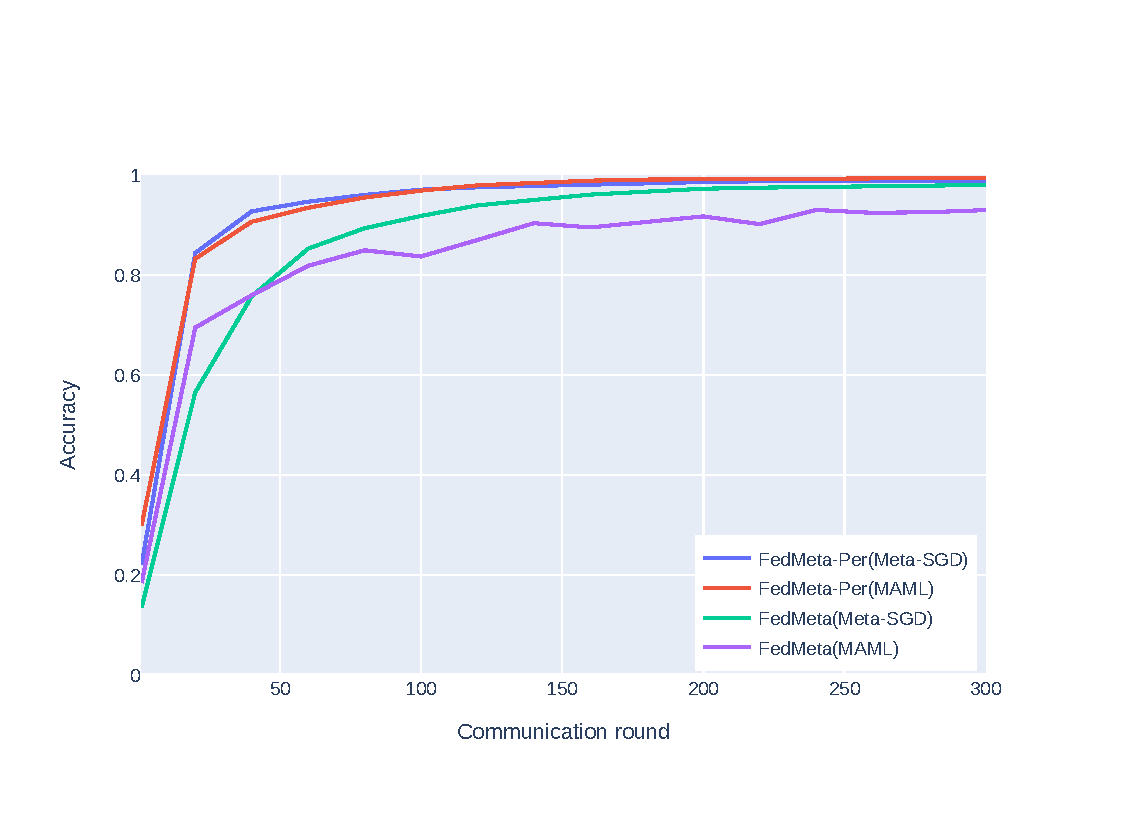
\includegraphics[width=\linewidth]{img/mnist_old_metaper.eps}
            \caption{MNIST, local client}\label{mnist_old_metaper}
        \end{subfigure}
        \begin{subfigure}{.49\textwidth}
            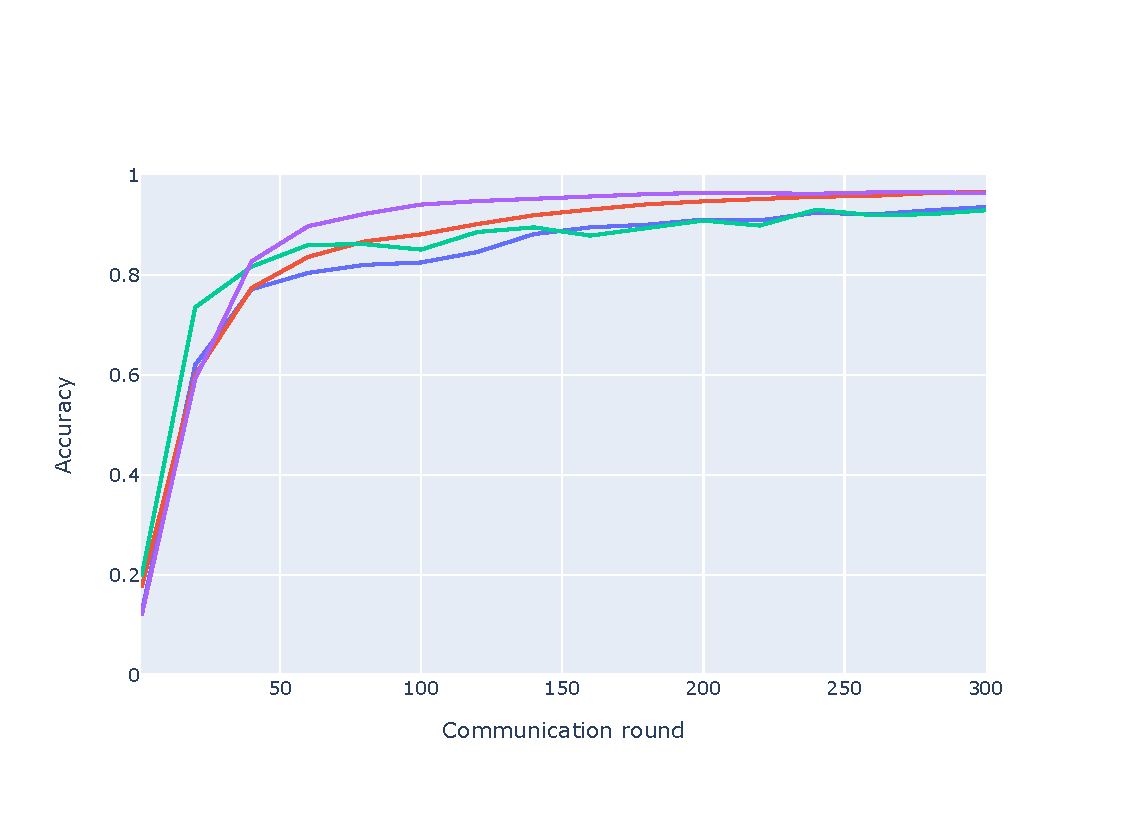
\includegraphics[width=\linewidth]{img/mnist_new_metaper.eps}
            \caption{MNIST, new client}\label{mnist_new_metaper}
        \end{subfigure}
    \end{subfigure}
    \begin{subfigure}{\textwidth}
        \centering
        \begin{subfigure}{.49\textwidth}
            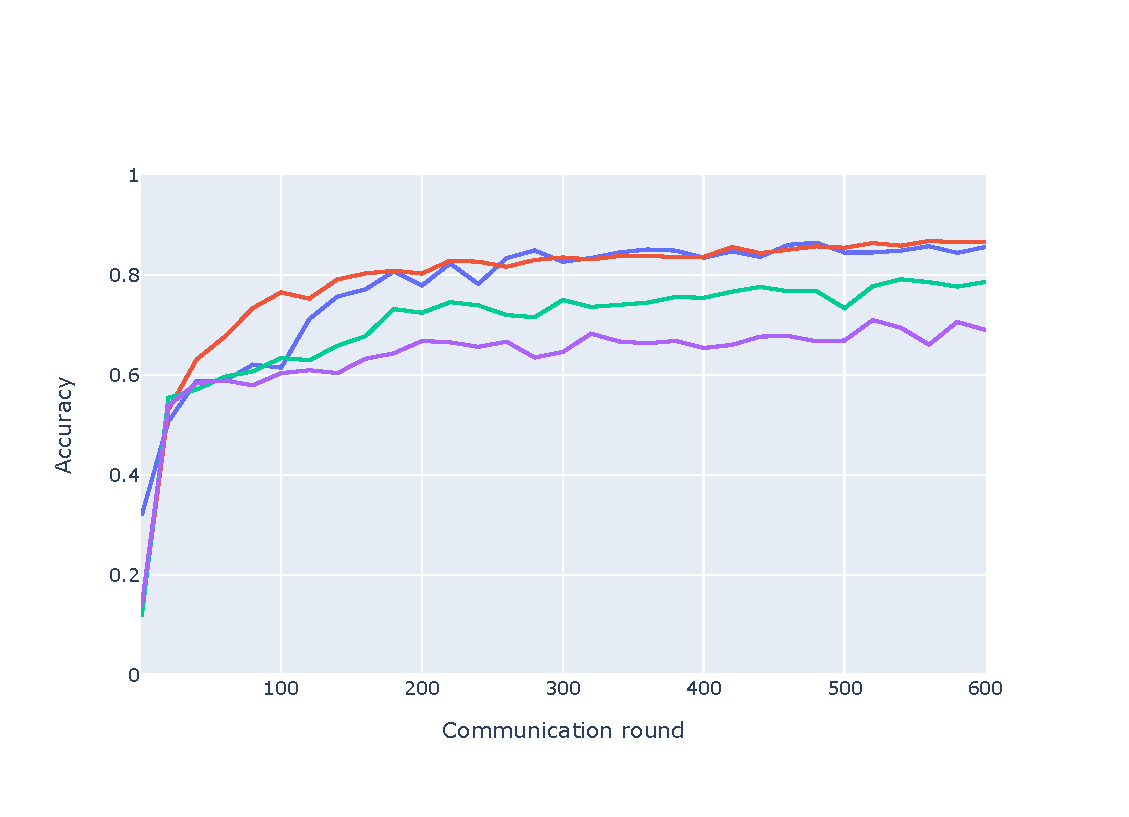
\includegraphics[width=\linewidth]{img/cifar_old_metaper.eps}
            \caption{CIFAR-10, local client}\label{cifar_old_metaper}
        \end{subfigure}
        \begin{subfigure}{.49\textwidth}
            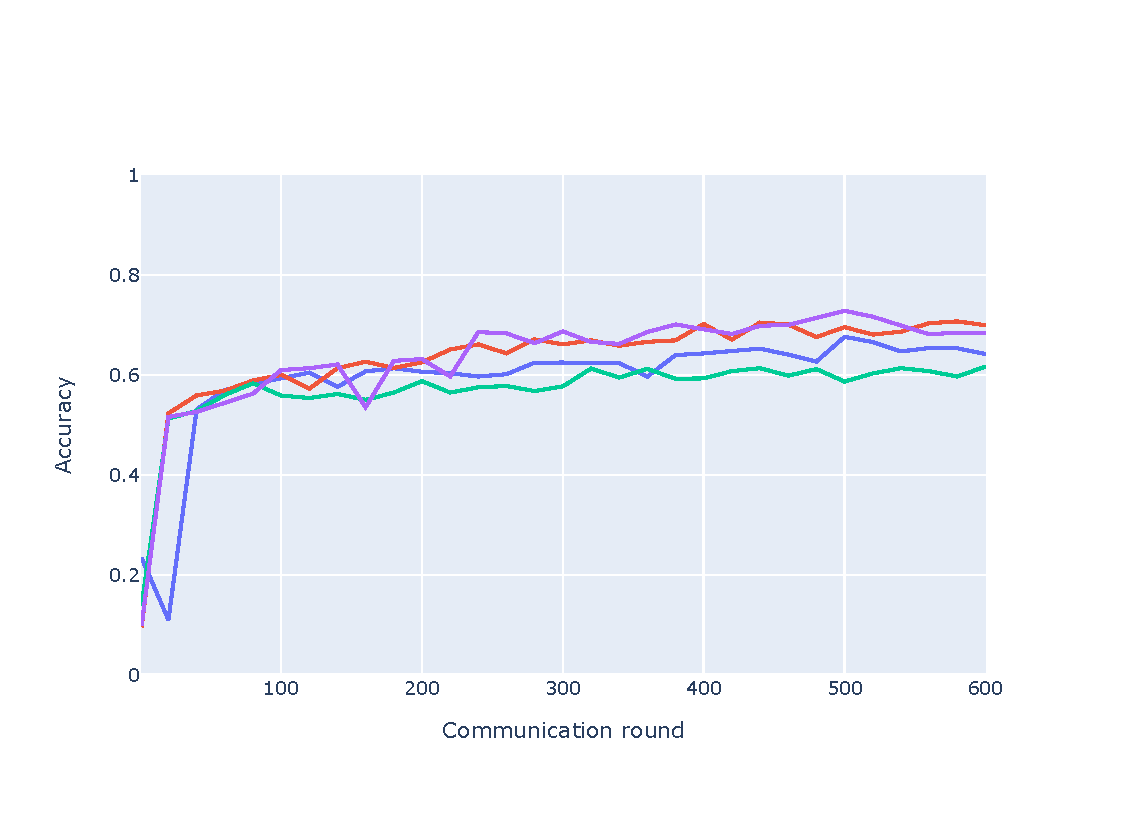
\includegraphics[width=\linewidth]{img/cifar_new_metaper.eps}
            \caption{CIFAR-10, new client}\label{cifar_new_metaper}
        \end{subfigure}
    \end{subfigure}
    \caption{$acc_{micro}$ of FedMeta-Per and FedMeta. The end result and convergence of FedMeta-Per is significantly higher than that of FedMeta on local clients. On new clients, even though FedMeta-Per reaches a higher value, the difference in convergence is not so great.} \label{fig:fedpermeta_vs_fedmeta}
\end{figure}

\begin{figure}[h]
    \centering
    \begin{subfigure}{\textwidth}
        \centering
        \begin{subfigure}{.49\textwidth}
            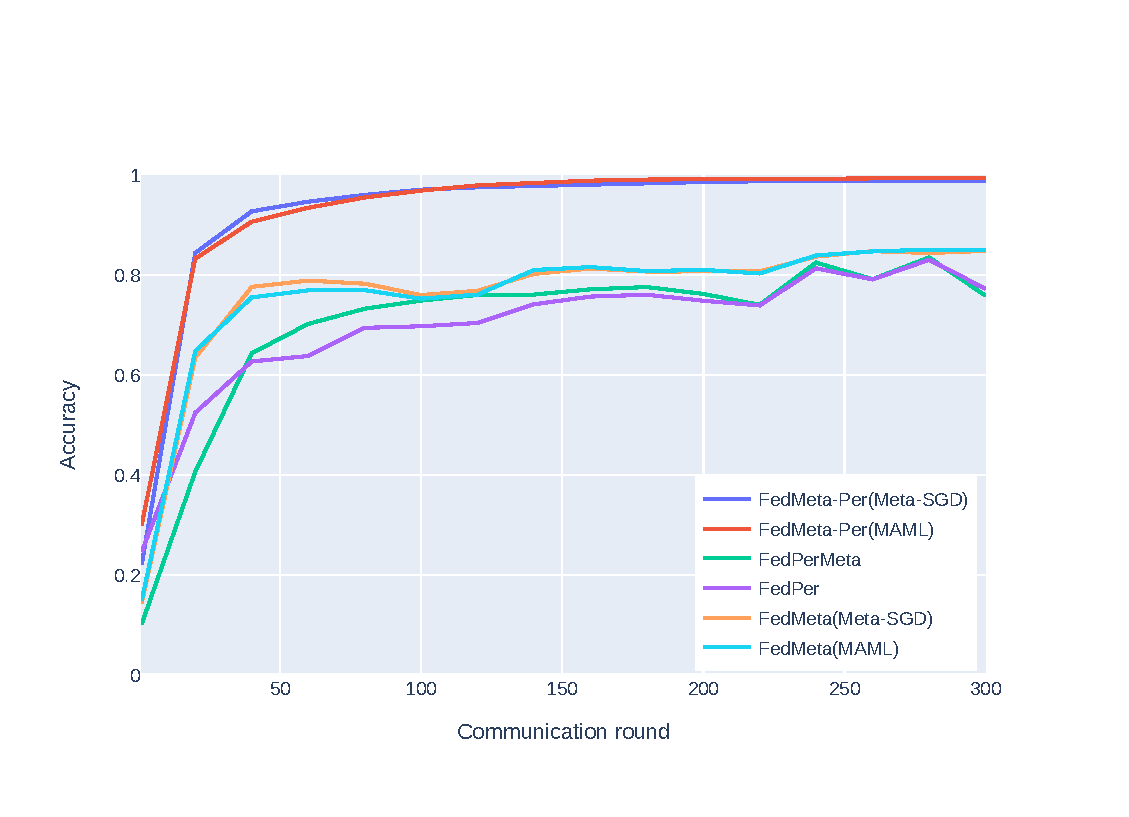
\includegraphics[width=\linewidth]{img/mnist_old_per.eps}
            \caption{MNIST, local client}\label{fig:mnist_old_per}
        \end{subfigure}
        \begin{subfigure}{.49\textwidth}
            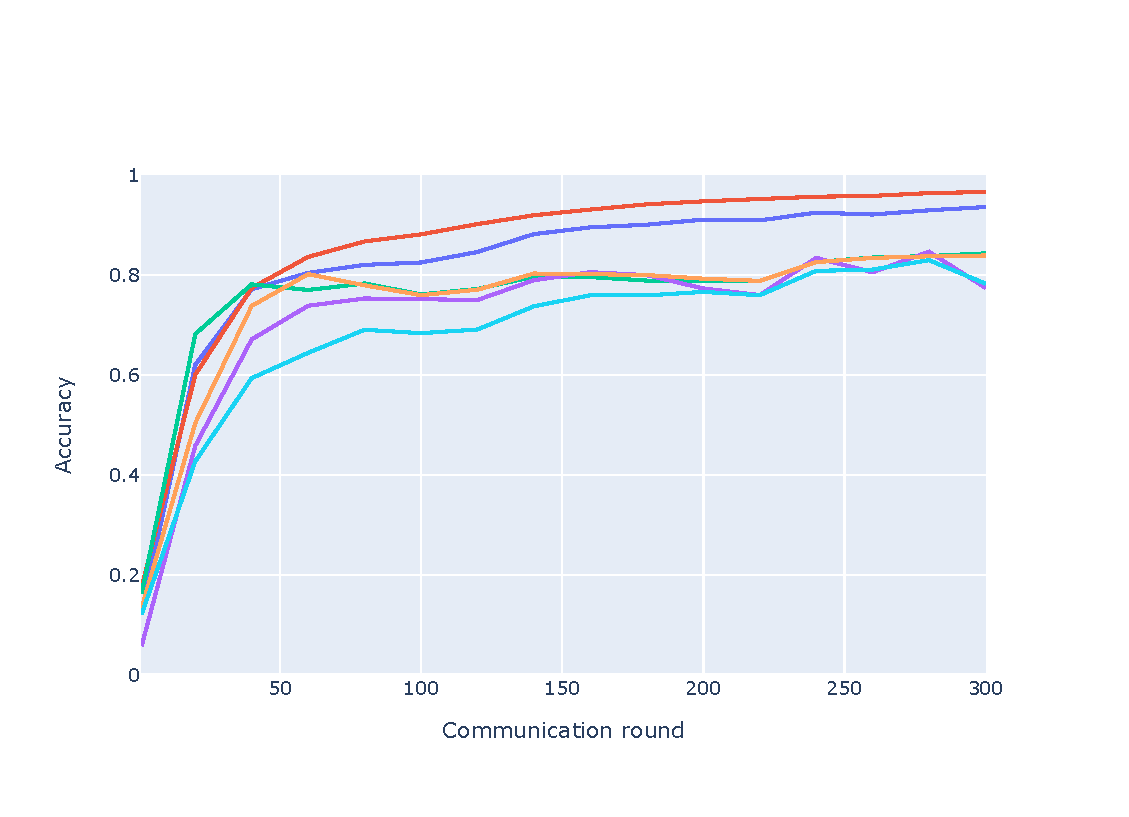
\includegraphics[width=\linewidth]{img/mnist_new_per.eps}
            \caption{MNIST, new client}\label{mnist_new_per}
        \end{subfigure}
    \end{subfigure}
    \begin{subfigure}{\textwidth}
        \centering
        \begin{subfigure}{.49\textwidth}
            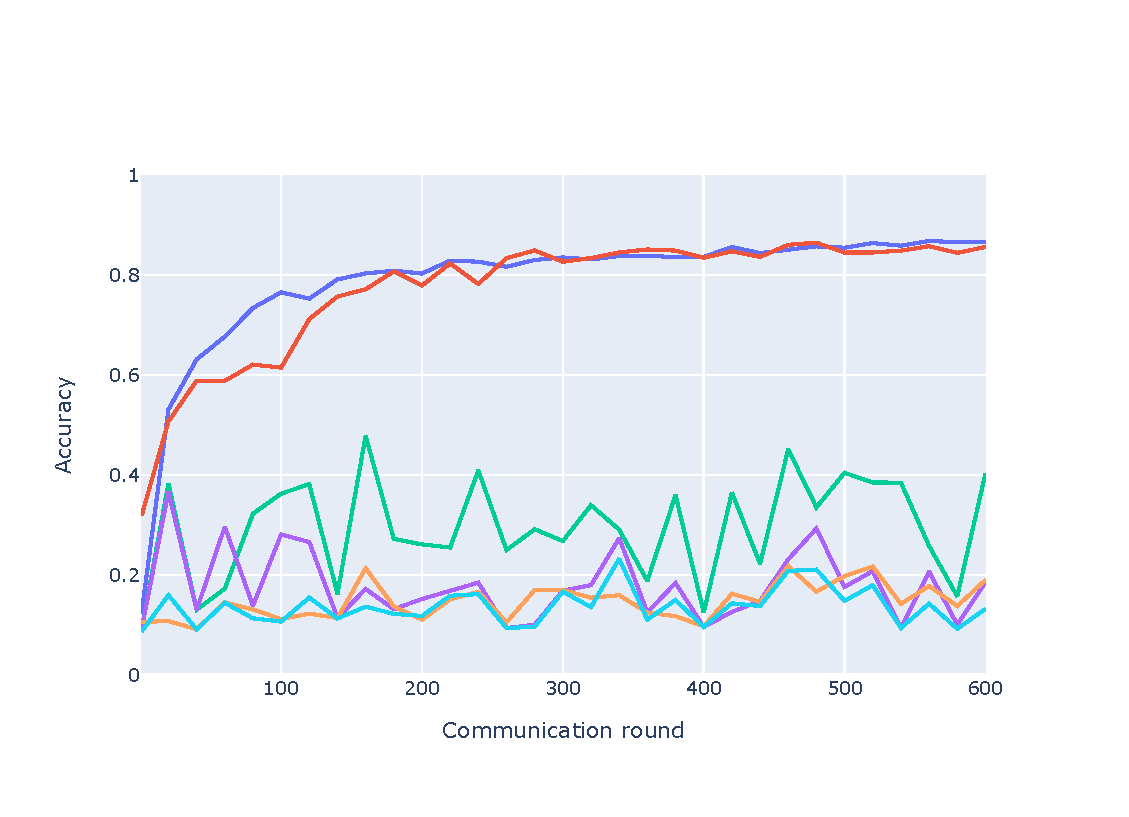
\includegraphics[width=\linewidth]{img/cifar_old_per.eps}
            \caption{CIFAR-10, local client}\label{cifar_old_per}
        \end{subfigure}
        \begin{subfigure}{.49\textwidth}
            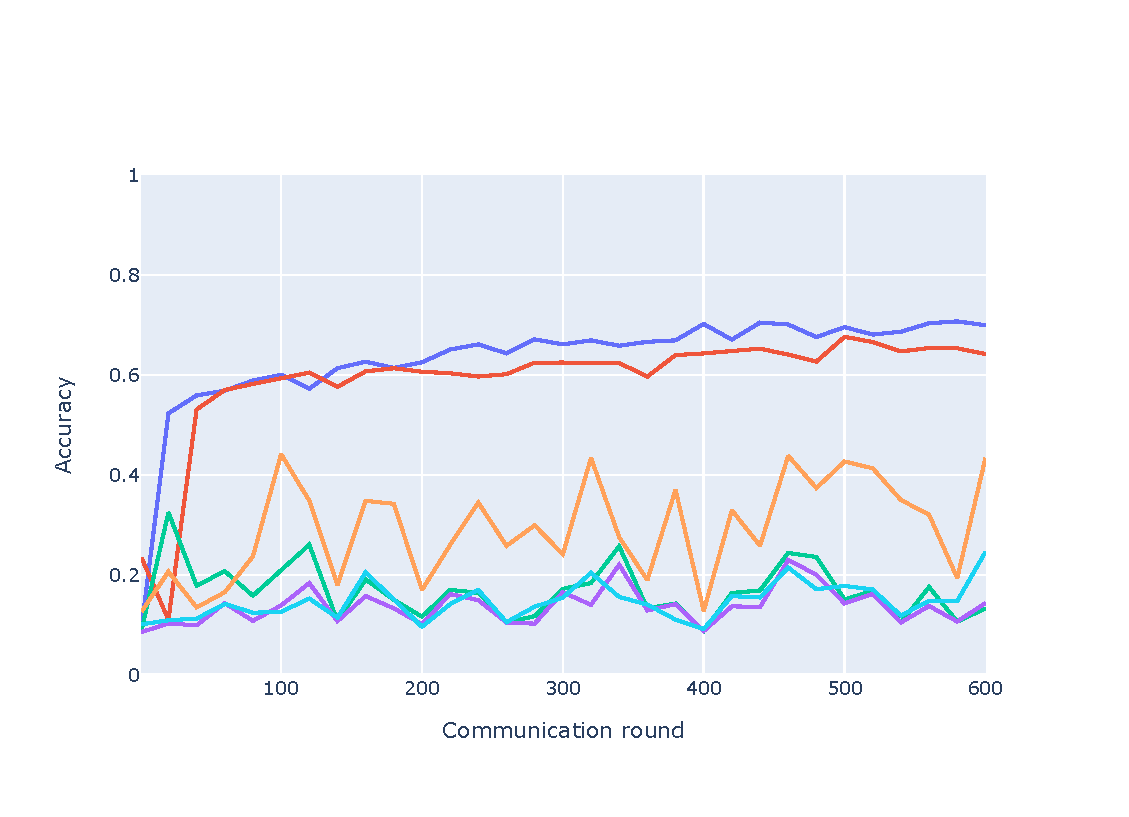
\includegraphics[width=\linewidth]{img/cifar_new_per.eps}
            \caption{CIFAR-10, new client}\label{cifar_new_per}
        \end{subfigure}
    \end{subfigure}
    \caption{$acc_{micro}$ of FedMeta-Per, FedAvg, FedAvgMeta, FedPer and FedPerMeta. FedMeta-Per's convergence and accuracy outperform the rest of the algorithms.} \label{fig:fedpermeta_vs_chicken}
\end{figure}

\textbf{Personalization ability}. Observing the standard deviation of the algorithms \codeword{FedMeta}, \codeword{FedAvg} and \codeword{FedPer} in Table \ref{tab:compare}, we can see the standard deviation in the results of \codeword{FedMeta} is much smaller than the rest of the algorithms. It shows that the personalization of the FL system has been improved many times thanks to the training of ML algorithms as well as the fine-tuning execution on the support set to capture the characteristics of a new data set. However, as mentioned above, this ability can be completely improved. With new suggestions during the inference phase, \codeword{FedMeta-Per} further reduces the standard deviations on the scales. Specifically, after combining the fine-tuning of the model with the support set of local data and maintaining the personalization layer for each client, the standard deviation of the local clients decreases from 4\% to 14\% on CIFAR-10 and from 1\% to 5\% on MNIST while the averages are still superior. On new clients, the mean values are higher but the standard deviation, in some cases, is not actually smaller than the previous algorithms. This is because the personalization layers in the deep neural network of new clients have not really matched that user yet. However, over time, when new clients participate in one or a few steps of global training, they will build up good personalization layers for themselves, resulting in the metrics reaching the same value as local clients.

\section{Conclusion}

Through the research process, we combine ML algorithms and PL techniques into the FL system, to improve the accuracy as well as the ability to personalize the machine learning model for each user of the system on non-IID data. Experimentally, we prove the effectiveness of the proposed algorithm \codeword{FedMeta-Per} compared with algorithms \codeword{FedAvg}, \codeword{FedPer}, and \codeword{FedMeta} over 50 users with two datasets, CIFAR-10 and MNIST. In which, it can be explained that achieving high results is based on two inherited factors: (1) - Fast adaptability to new data set of the proposed algorithm inherited from ML algorithms, (2) - High personalization ability for each user inherited from personalization layers of PL technique and model fine-tuning on the support set of ML algorithms.

In the future, bilevel optimization-based algorithms (\codeword{FO-MAML} \cite{finn2017model}, \codeword{iMAML} \cite{rajeswaran2019meta}, \codeword{Reptile}) can be integrated into the system. The search and clustering of users so that each user finds the best set of partial parameters should also be further studied to increase the performance of the system. In addition, the issue of information security between the server and the client should also be considered to make the system more practical.
\clearpage

% \begin{figure}[H]
%     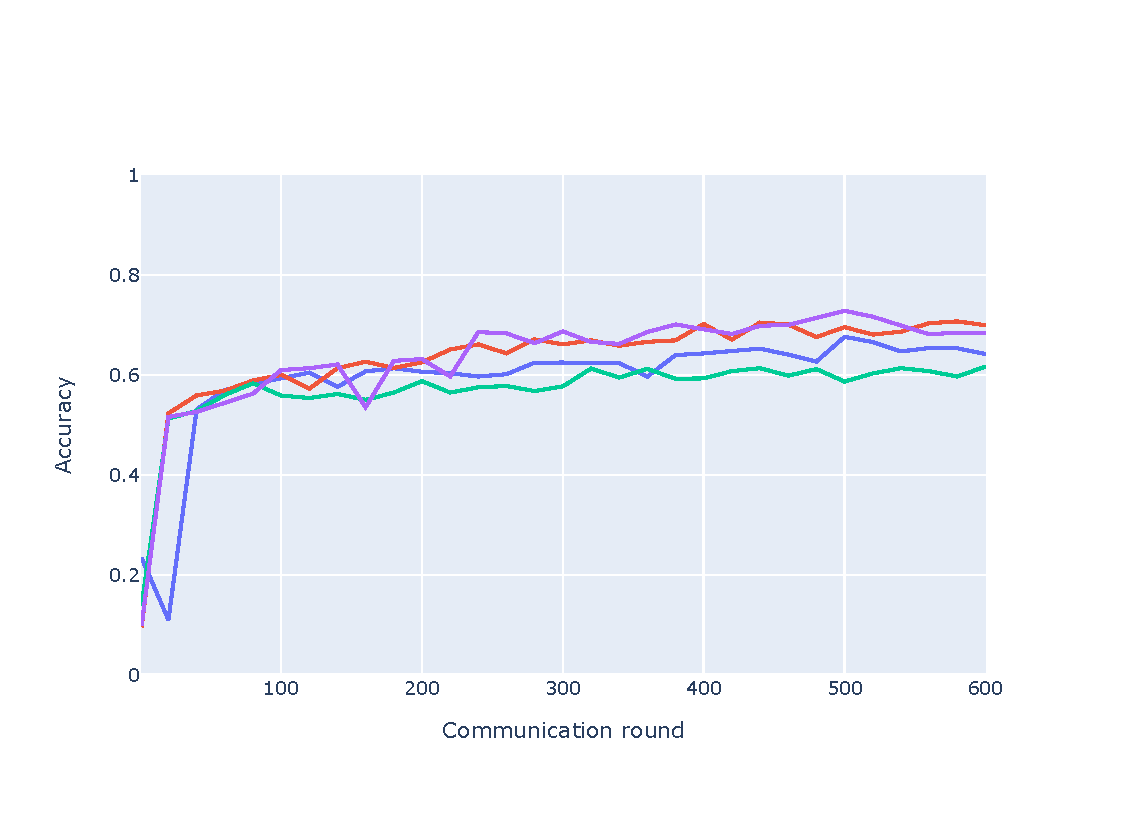
\includegraphics[width=\textwidth]{img/cifar_new_metaper.eps}
%     \caption{A figure caption is always placed below the illustration. Please note that short captions are centered, while long ones are justified by the macro package automatically.} \label{fig1}
% \end{figure}
%
% the environments 'definition', 'lemma', 'proposition', 'corollary',
% 'remark', and 'example' are defined in the LLNCS documentclass as well.

\appendix
\section{Experimental Details}
\label{appendix}

\subsection{Model Architecture}
\label{model_architecture}

The study uses two simple models for feature extraction and data classification for the CIFAR-10 and MNIST datasets.

\textbf{CIFAR-10.} The model takes input images of size $(32\times32\times3)$. Two convolution layers (kernel of size $(5\times5)$, channel numbers of $6$ and $16$ respectively) are used for feature extraction. Following each convolution layer is a \codeword{MaxPooing} layer of size $(2\times2)$. The classifier consists of three linear layers whose outputs are $120$, $84$ and $10$ respectively. The activation functions used are \codeword{ReLU} and \codeword{Softmax}.

\textbf{MNIST.} The model receives flattened input images of size $(1\times784)$. Use two linear layers with outputs of 100 and 10, respectively. The activation functions used are \codeword{ReLU} and \codeword{Softmax}.

\subsection{Hyper-parameters Searching}

The hyper-parameters of the FL system of the study include: the number of clients participating in training in a global training step ($\#clients/round$), number of local training steps ($\#epochs $), number of global training steps ($\#rounds$), amount of data in a data batch ($batch\_size$), number of personalization layers for algorithms using PL techniques ($\# per\_layers$) and the learning rates used in the optimization of deep neural networks by mini batch gradient descent.

To accommodate the limited configuration client hardware in the Horizontal FL scenario, we limits $\#epochs=1$ and $batch\_size=32$. From the survey of FL experiments in recent studies, the number of clients participating in global training was selected as 2, 5, and 10, respectively. In which, $\#clients/round=5$ gives a higher result and consumes an acceptable computational cost. $\#per\_layers$ is searched in $\{1,2,3\}$ (calculated from the last linear layer). Experimental results show that using the last linear layer as the personalization layer gives the best results. The learning rates are presented in Table \ref{tab:hyper_param}.

% Except for the learning rate of each algorithm, the above hyper-parameters are kept fixed during training. Table \ref{tab:fixed_hyper_param} summarizes these hyper-parameters values.

% \begin{table}[h]
%     \centering
%     \caption{Fixed hyper-parameters in FL system}
%     \label{tab:fixed_hyper_param}
%     % \resizebox{\linewidth}{!}{%
%     \begin{tabular}{l|ccccc} 
%     \toprule
%              & \#clients/round    & \#epochs           & \#rounds & batch\_size         & \multicolumn{1}{l}{\#per\_layers}  \\ 
%     \hline
%     MNIST    & \multirow{2}{*}{5} & \multirow{2}{*}{1} & 300      & \multirow{2}{*}{32} & \multirow{2}{*}{1}                \\
%     CIFAR-10 &                    &                    & 600      &                     &                                   \\
%     \bottomrule
%     \end{tabular}
%     % }
% \end{table}

\begin{table}[h]
    \centering
    \caption{Tuning learning rate for algorithms. Empty cells indicate that hyper-parameters cannot be found for the model to converge.}
    \label{tab:hyper_param}
    % \resizebox{\linewidth}{!}{%
    \begin{tabular}{l|cc} 
    \toprule
    \begin{tabular}[c]{@{}l@{}}\\\end{tabular} & CIFAR-10           & MNIST                                             \\ 
    \hline
    FedAvg, FedAvgMeta                         & -                  & $10^{-5}$                                      \\
    FedPer, FedPerMeta                         & -                  & $10^{-5}$                                      \\
    FedMeta(MAML) ($\alpha,\beta$)             & $(0.01, 0.001)$    & $(0.001, 0.001)$                                \\
    FedMeta(Meta-SGD)($\alpha,\beta$)          & $(0.001, 0.001)$   & $(0.001, 5\times 10^{-4})$  \\
    FedMeta-Per(MAML)($\alpha,\beta$)          & $(0.001, 0.005)$   & $(0.001, 0.001)$                                \\
    FedMeta-Per(Meta-SGD)($\alpha,\beta$)      & $(0.01,0.01)$      & $(0.001, 5\times 10^{-4})$  \\
    \bottomrule
    \end{tabular}
    % }
\end{table}

\subsubsection*{Acknowledgements} This research is funded by University of Science, VNU-HCM under grant number CNTT 2022 - 09.
\clearpage
% ---- Bibliography ----
%
% BibTeX users should specify bibliography style 'splncs04'.
% References will then be sorted and formatted in the correct style.
%
\bibliographystyle{splncs04}
\bibliography{mybibliography}
\clearpage

% \begin{thebibliography}{8}
% \bibitem{ref_article1}
% Author, F.: Article title. Journal \textbf{2}(5), 99--110 (2016)

% \bibitem{ref_lncs1}
% Author, F., Author, S.: Title of a proceedings paper. In: Editor,
% F., Editor, S. (eds.) CONFERENCE 2016, LNCS, vol. 9999, pp. 1--13.
% Springer, Heidelberg (2016). \doi{10.10007/1234567890}

% \bibitem{ref_book1}
% Author, F., Author, S., Author, T.: Book title. 2nd edn. Publisher,
% Location (1999)

% \bibitem{ref_proc1}
% Author, A.-B.: Contribution title. In: 9th International Proceedings
% on Proceedings, pp. 1--2. Publisher, Location (2010)

% \bibitem{ref_url1}
% LNCS Homepage, \url{http://www.springer.com/lncs}. Last accessed 4
% Oct 2017
% \end{thebibliography}

\end{document}
